\section{High-Level Overview}
\label{sec:overview}

\begin{figure}[ht]
    \centering
    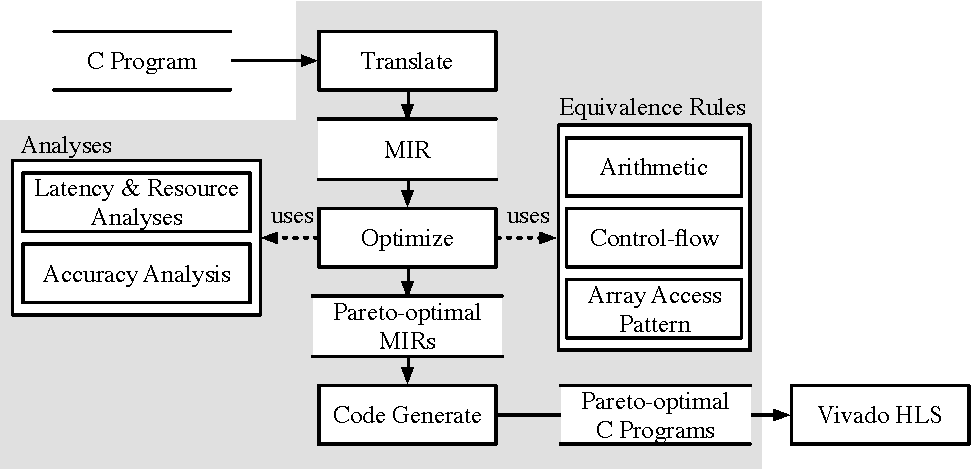
\includegraphics[width=\linewidth]{overview}
    \caption{%
        An overview of our automatic program optimization process. The shaded
        region shows our internal tool flow.
    }\label{fig:overview}
\end{figure}

We start by introducing a high-level overview of our program optimization
process (Fig.~\ref{fig:overview}).  Our automatic optimization process starts
by taking as an input, the original numerical program written in C, and
translates it into an MIR\@.  An MIR is a directed acyclic graph (DAG), and
it serves as an abstract representation of the original program.  It discards
information about \emph{how} a program is executed, which is dependent on
how the program is structured in C, but retains the \emph{effect} of program
execution, keeping only the structure that leads to the final results.  This
procedure, explained in detail in Sec.~\ref{sec:intermediate}, greatly reduces
the number of program transformations we need to explore.  We then discover
equivalent MIRs using our efficient optimization procedure discussed in detail
in Sec.~\ref{sec:structural_optimization}.  The optimized C programs can then
be generated from the MIRs, using the \SOAP{} framework's code generation
routines, to be synthesized in Vivado HLS to obtain RTL implementations.

As we apply transformation rules to discover equivalent MIRs, we estimate
latency, resource usage and analyze round-off errors for each MIR we have
discovered.  Non-Pareto-optimal MIRs---the ones with all three performance
metrics (latency, resource usage and accuracy) worse than any other MIRs---are
pruned immediately to keep the size of total MIRs discovered tractable.
Sec.~\ref{sec:performance_analysis} explains in depth how we analyze latency,
resource usage and accuracy.
